\documentclass[11pt,a4paper]{article}
\usepackage[margin=2.2cm]{geometry}
\usepackage{amsmath,amssymb}
\usepackage{siunitx}
\usepackage{booktabs}
\usepackage{xcolor}
\usepackage{microtype}
\usepackage{enumitem}
\usepackage{tcolorbox}
\usepackage{graphicx}
\definecolor{ink}{HTML}{14231B}\definecolor{accent}{HTML}{0F3D2A}
\tcbuselibrary{skins}
\newtcolorbox{key}{colback=accent!6,colframe=accent,boxrule=0.6pt,arc=2pt,left=6pt,right=6pt,top=4pt,bottom=4pt}
\sisetup{per-mode=symbol,group-separator={\,}}
\setlength{\parindent}{0pt}\setlength{\parskip}{6pt}
\renewcommand{\arraystretch}{1.25}

\title{\textbf{Slide 8: the ADC input and the ADS7057}\\\large A 14-bit ADC and the network that feeds it}
\author{ADS7057 test board v3 \quad ---\quad study notes}\date{}
\begin{document}\maketitle\vspace{-1.2em}
\section{The circuit}
\begin{center}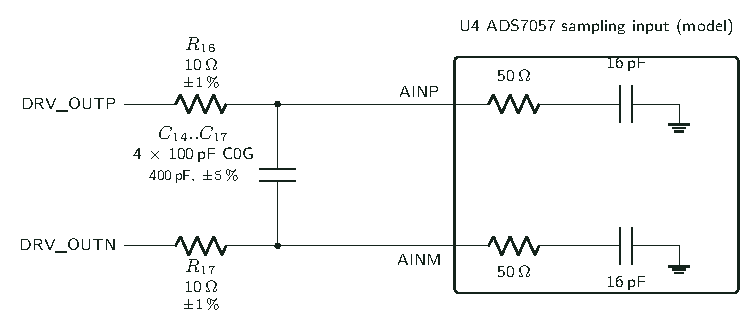
\includegraphics[width=0.98\textwidth]{s08_circuit.pdf}\end{center}
R16 and R17 (\SI{10}{\ohm}) and the four \SI{100}{pF} C0G capacitors C14 to C17 (\SI{400}{pF}) sit between the driver and the ADC. Inside the ADC each input leg is a switch of about \SI{50}{\ohm} in series with a \SI{16}{pF} sampling capacitor.

\section{What one code means}
Full scale is $\pm$AVDD, and AVDD is also the reference. The code is 14-bit two's complement, so
\[
\text{LSB}=\frac{2\,\text{AVDD}}{2^{14}}=\frac{6.6\,\text{V}}{16384}=\SI{0.403}{mV}.
\]
A \SI{120}{mV} event at the head becomes about \SI{0.5}{V} at the ADC, about 1280 codes, 16\,\% of the positive range. The sensor noise is 38 to 47 LSB rms, the board adds 0.2 LSB and the ADC adds about 0.6 LSB. The sensor decides the noise floor.

\section{The kickback}
When the sampler closes, the \SI{16}{pF} capacitor is connected to a node that holds the previous sample. It takes a charge from the input. For the worst step of \SI{0.56}{V}:
\[
Q=C_s\,\Delta V=16\,\text{pF}\times0.56\,\text{V}=\SI{9.0}{pC}.
\]
The \SI{400}{pF} bucket supplies this charge, so the input node dips by
\[
\Delta V=\frac{Q}{C_\text{bucket}}=\frac{9.0\,\text{pC}}{400\,\text{pF}}=\SI{22.4}{mV}\;(\approx 56\ \text{LSB}).
\]
The datasheet asks for at least 20 times the sampling capacitance ($16\times20=\SI{320}{pF}$). The board has 25 times.

\section{Settling}
The two \SI{10}{\ohm} resistors recharge the bucket. First-order model: $\tau=(R_{16}+R_{17})\,C=20\,\Omega\times400\,\text{pF}=\SI{8}{ns}$, a pole at $1/(2\pi\tau)=\SI{19.9}{MHz}$, far above the band. The dip decays as $e^{-t/\tau}$. It reaches half an LSB (\SI{0.2}{mV}) after
\[
t=\tau\ln\frac{22.4\,\text{mV}}{0.2\,\text{mV}}=8\,\text{ns}\times4.7=\SI{38}{ns}.
\]
\begin{center}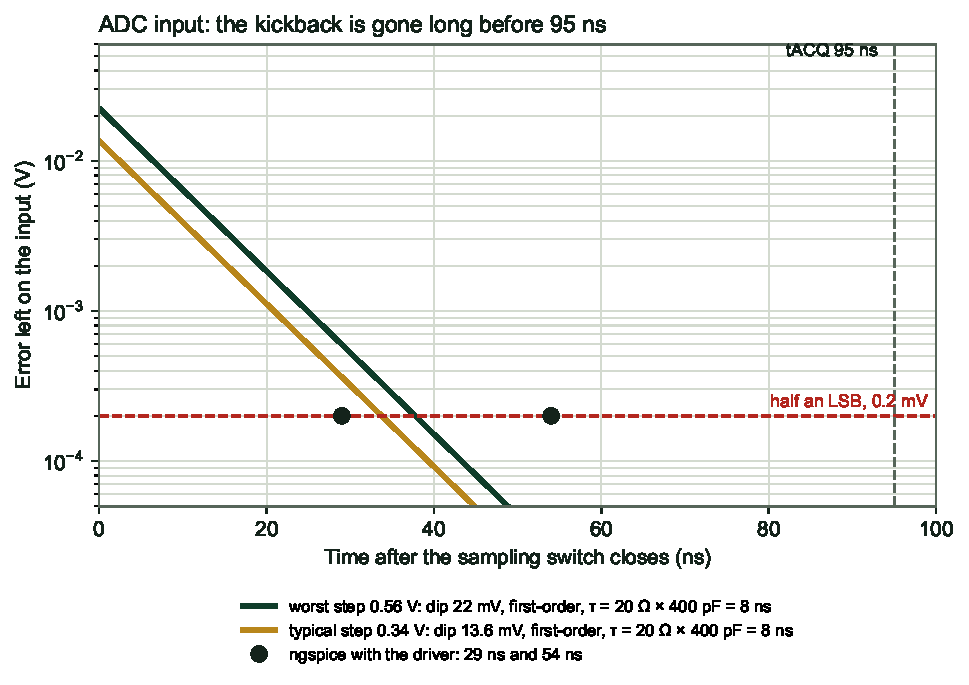
\includegraphics[width=0.82\textwidth]{s08_graph.pdf}\end{center}
The ngspice run with the real driver gives \SI{29}{ns} for a typical step and \SI{54}{ns} for the worst step. The ADC allows \SI{95}{ns}. The hand estimate (\SI{38}{ns}) and the simulation are the same size, and both leave margin.

\section{Decoupling}
AVDD has \SI{4.7}{\micro F} (C18) and \SI{100}{nF} (C22). DVDD has \SI{1}{\micro F} (C19) and \SI{100}{nF} (C20). C22 is \SI{2.4}{mm} and C18 \SI{2.7}{mm} from the ADC. The \SI{100}{nF} parts for DVDD sit farther (\SI{4.5}{mm}), which is a point to improve.

\begin{key}
The ADS7057 is 14 bit, up to \SI{2.5}{MSPS}, $\pm0.9$ LSB INL, 79.6 dB SNR at \SI{2}{kHz}. It samples on the falling edge of CS.
\end{key}
\end{document}
